\documentclass{standalone}
\usepackage{pgfplots}
\pgfplotsset{compat=newest}
\begin{document}
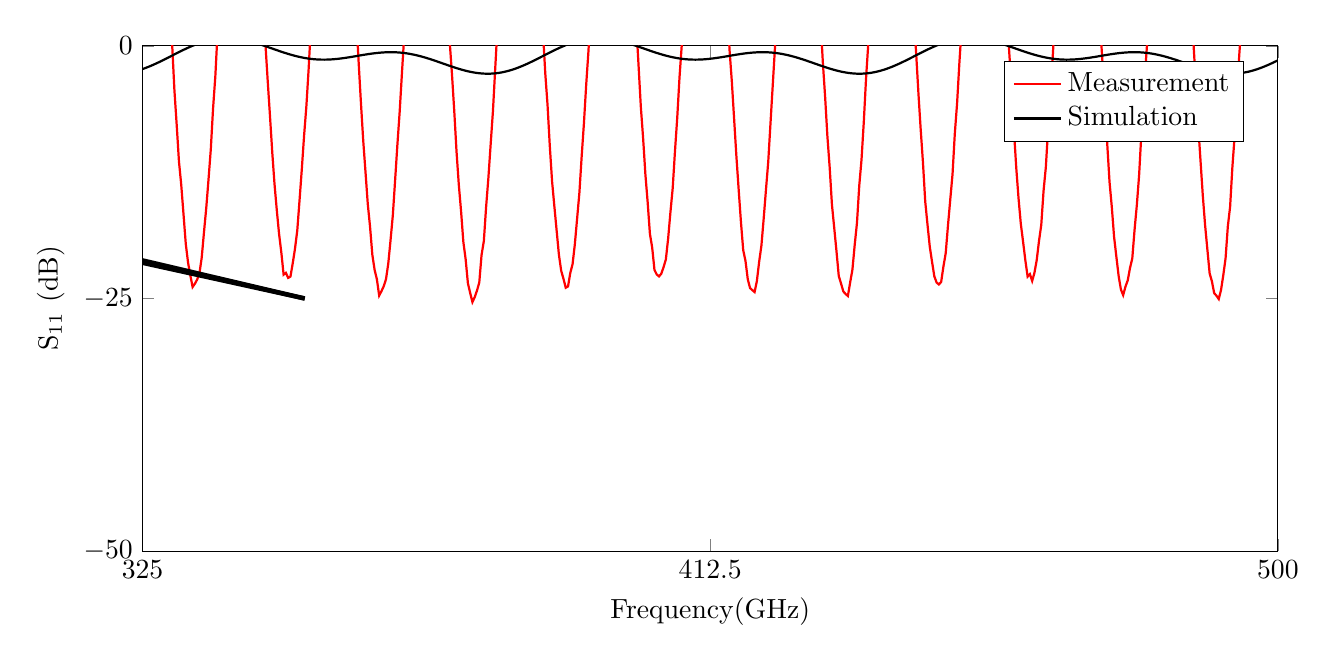
\begin{tikzpicture}[scale=1]
    \begin{axis}[
        xlabel=Frequency(GHz),
        ylabel={S$_{11}$ (dB)},
        width=16cm,
        height=8cm,
        xmin=325,
        xmax=500,
        ymin=-50,
        ymax=0,
        xtick={325,412.5,500},
        ytick={-50,-25,0},
        legend pos=north east,
        title style={align=center},
        legend style={nodes=right},
        legend cell align=left,
        legend entries={
            Measurement,
            Simulation},
        xmajorgrids=false,
        grid=none,
        ]
        \addplot[
            domain=325:500,
            samples=500,
            color=red,
            thick,
        ] {(-25*sin(8*pi*x)+cos(2*pi*x)+1)+rand*0.5};
        \addplot[
            domain=325:500,
            samples=500,
            color=black,
            thick,
        ] {-sin(4*pi*x)+cos(2*pi*x)-1};
        \draw[->,ultra thick] (axis cs:350, -25) -- node[above=0.2cm] {Open-ended wg.\ probe} ++(-15pt, 0);
        \draw[->,ultra thick] (axis cs:350, -25) -- node[right=0.3cm, text=black] {Diagonal horn} ++(0, -15pt);
    \end{axis}
\end{tikzpicture}
\end{document}